\chapter{Proposed Work and Planning}
\label{chapter:PWP}

The proposed work for the dissertation consists in the development of an
automatic compiler of DNN description into DeepVersat / IOB-RV32 C++ code. The
purpose of this work is to be able to run any state of the art CNN on the Deep
Versat system with no effort on the user side, allowing the design and
architectural exploration.

For the proof of concept stage, Darknet and Caffe will be the frameworks chosen
to be supported by the compiler. DeepVersat can customized with the number of
layers, numbers of each FU type and other options. Hence, the compiler must be
able to take the configurations into account when producing computational
datapaths for DeepVersat.

\section{Flowchart}

\begin{figure}[!htb]
    \centering
    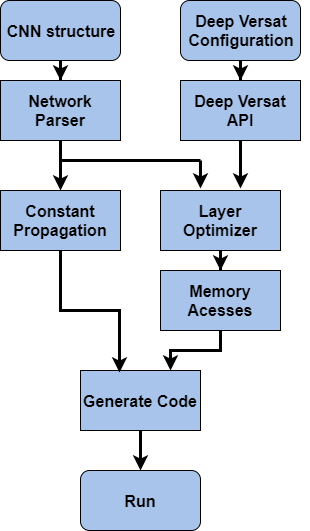
\includegraphics[width=0.5\textwidth]{Figures/flowchart.png}
    \caption{Flowchart of the software architecture}
    \label{figure:flowchart}
\end{figure}



Figure~\ref{figure:flowchart} presents the flowchart of the system to be developed. The steps
of the algorithm are explained in the next paragraphs.


The frameworks to be adopted for the Configuration files are Darknet~\cite{Darknet} and Caffe~\cite{caffe}.The former is to be adopted
to support other dissertations that use Yolov3~\cite{yolov3} while the latter is one of the most used frameworks as seen in table~\ref{table:toolflow}.Also,
unlike some other frameworks, Caffe is also based on Google's Protocol Buffers serialization library which is easier to work with.
The goal after parsing is for the end result to be framework abstract, so other frameworks can be implemented into the compiler.
When parsing the network, the compiler propagates the constants i.e input and output parameters of each layer.

With the network defined and DeepVersat deployed, each layer of the network can be mapped onto Versat (Layer Optimizer). Because the input size of each layer
can be bigger than a Versat Memory, certain optimizations such parallelism exploration must be made to guarantee that each network layer is processed as efficiently as possible. 
How much performance can be extracted depends on the DeepVersat Configuration that is deployed, that is, performance per functional Unit, how many per Versat core and
total number of cores.

Memory accesses are all the operations to manage data from external memory to the RISC-V core and to the DeepVersat Cores and vice-versa.
Finally the compiler generates the code for the CPU that controls DeepVersat.
\newpage
\section{Workplan}


\begin{figure}[!htb]
    \centering
    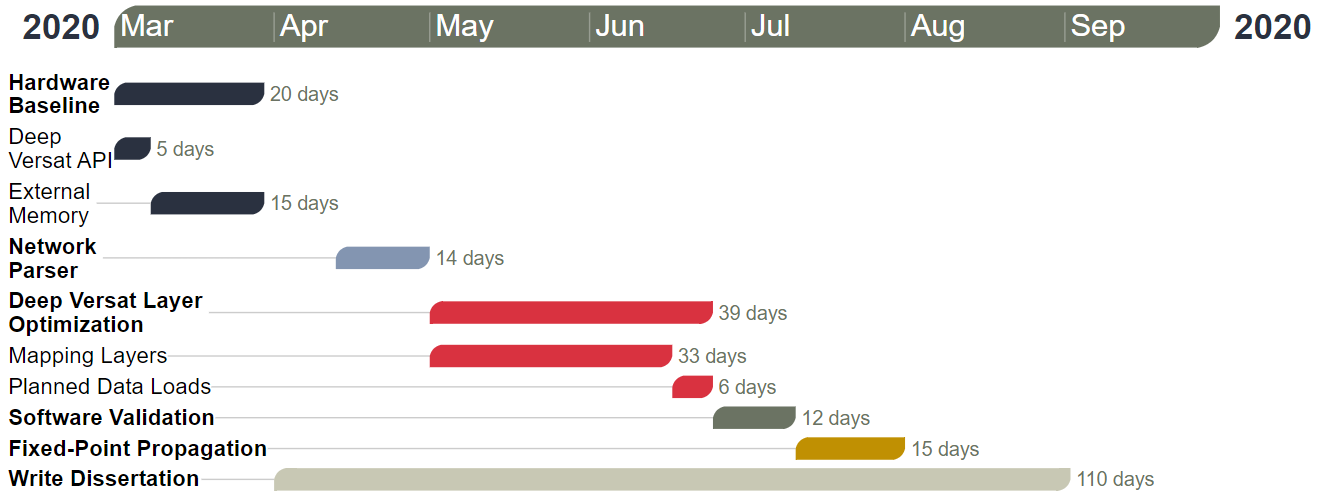
\includegraphics[width=1\textwidth]{Figures/gant22.png}
    \caption{GANT chart of Proposed Work}
    \label{figure:gant}
\end{figure}

In Fig~\ref{figure:gant}, a GANT chart with the proposed schedule for the
planned work is presented. In the GANT chart, 20 days will be used to deploy DeepVersat system and study external memory use and testing
memory accesses with the RISC-V core and with DeepVersat. Then the core components in~\ref{figure:flowchart} are designed. Afterwards
software validation and testing is done to ensure the compiler works as intended. Finally, because DeepVersat uses Integer functional units, fixed-point arithmetic
is used instead. Fixed-Point formats are prone to overflow or underflow due to the fixed range it offers, thus 15 working days are allocated to
make sure the outputs of any CNN network are valid and according to expected results. 






